% ---------------------------------------------------------------------------
% Ingestion mapping and phi-relative soundness, for the main direction
% (Datadog -> PromQL). Requires \sem, \Lang from macros.tex.
% Numbers come from notebook 02 and data/raw/anchored/ (scripts/verify_anchored.py).
% ---------------------------------------------------------------------------

\subsection{Ingestion and \texorpdfstring{$\phi$}{phi}-relative soundness}
\label{sec:ingestion}

\paragraph{Scope: forward portability.}
The goal is portability of \emph{queries going forward}: once an organization
dual-writes (or switches) its telemetry, a translated query must mean the same thing
as the original on the data each system receives from then on. Migrating stored history
is out of scope. The two systems still do not store the same thing, however, so
soundness must be stated relative to how each ingests data.

\begin{definition}[Ingestion mapping]\label{def:phi}
A Prometheus counter series $s=(\lambda,\langle (t_1,v_1),\dots,(t_n,v_n)\rangle)$ stores
cumulative values. Datadog stores \texttt{COUNT} points that are per-interval deltas. For a
reset policy $\rho\in\{\mathsf{zero},\mathsf{clamp}\}$ define
\[
\phi_\rho(s) = \big(\lambda,\ \langle (t_i,\ \delta_\rho(v_{i-1},v_i)) : 2\le i\le n \rangle\big),
\]
\[
\delta_\rho(u,v)=\begin{cases}
v-u & v\ge u\\
v & v<u,\ \rho=\mathsf{zero}\quad\text{(restarted from $0$, as PromQL assumes)}\\
0 & v<u,\ \rho=\mathsf{clamp}\quad\text{(the decrease contributes nothing)}
\end{cases}
\]
Every series that is not a counter --- a gauge, and the $\mathsf{delta}$ kind
Definition~\ref{def:model} also admits --- maps by the identity, so $\phi_\rho$ is total
on $\mathcal{D}$ and the statements below may quantify over all of it.
$\phi_\rho$ extends to databases series by series:
$\phi_\rho(D)=\{\phi_\rho(s): s\in D\}$. The first sample is omitted. For the agent path
this paper models, that is read from the agent's source rather than from
documentation~\citep{ddagent}, as Remark~\ref{rem:rho} describes; Datadog documents the
same rule for its OTLP path, where a cumulative monotonic sum is differenced and the
first point stored but omitted~\citep{ddotlp}. Every claim below names the
$\rho$ it holds for.
\end{definition}

\begin{remark}[Which $\rho$, and how we know]\label{rem:rho}
Datadog's documentation does not say what becomes of a counter decrease. Its agent is
open source, so the question can be answered by reading it~\citep{ddagent}, and then put
to a running one; both were done and they agree. The reading first.

The conversion carries a per-sample flag. With the flag set, a
sample below its predecessor contributes its own value, on the agent's stated assumption
that the counter restarted from zero --- this is $\delta_{\mathsf{zero}}$ term for term.
With the flag clear, the decrease contributes nothing and the point is still emitted,
which is $\delta_{\mathsf{clamp}}$. The OpenMetrics check sets the flag after every
successful scrape, so the ingestion path this paper models is $\phi_{\mathsf{zero}}$ from
its second scrape onward: the policy PromQL's own reset handling assumes.

Both branches above are thus implemented, and a third that an earlier draft of this
section offered --- discarding the interval outright --- is not, at least not as a reset
policy. Discarding is instead what happens at the \emph{start} of a series, where there is
no predecessor to difference against. A failed scrape is the interesting case: it clears
the flag, so the next interval is converted under $\mathsf{clamp}$ rather than
$\mathsf{zero}$, and is dropped altogether if the aggregator's stored predecessor has
expired in the meantime. Either way a transient failure perturbs $\phi(D)$ in a way
nothing applied to $D$ reproduces, and Proposition~\ref{prop:admissible} gives no warning,
because the discrepancy is between the two stored databases rather than between two
queries. No refusal can flag it and no translation can repair it.

Reading the agent establishes what it intends to send, not what the backend stores, and
the two are different claims. E1 closes the gap by putting a real agent in the loop. A
local endpoint exposes a counter that climbs by one per scrape to $1000$ and then, inside
one rollup bucket, drops to $100$; a Datadog Agent runs an OpenMetrics check against it
and a Prometheus scrapes the same endpoint. Over the bucket holding the reset Datadog
stores $\mathbf{103}$ across four points --- the increment before the reset, the new
value reported as the reset interval's own count, and the two increments after it. That
is $\delta_{\mathsf{zero}}$ and nothing else: $\mathsf{clamp}$ predicts $3$ over four
points, discarding the interval predicts $3$ over three, and a backend keeping the signed
difference predicts $-897$. The four predictions were recorded before the run and are
regression-tested in \texttt{tests\slash test\_reset.py}. A second counter resetting to
exactly $0$ rather than $100$ reads $3$, which is what $\mathsf{zero}$ requires and rules
out a special case at zero; a third that never resets reads four increments of one in
every bucket, which is what shows the run is reading the bucket it means to.
\end{remark}

\begin{remark}[$\phi_\rho$ and the flush interval]\label{rem:flush}
$\phi_\rho$ differences consecutive \emph{samples}, and the agent aggregates samples
into the interval it flushes. An earlier version of this remark inferred from the source
that the two part company as soon as a flush holds more than one sample: a decrease
appeared to \emph{overwrite} what the interval had accumulated rather than adding to it,
so a flush holding an increase and then a reset should report the post-reset value alone,
where $\phi_{\mathsf{zero}}$ keeps both. The agent's default scrape and flush intervals
are both $15$\,s, which would make the question moot in the default configuration and
was the reason it went untested.

Put to a running agent, it does not happen --- though not quite for the reason the run
was designed to test, and the difference is worth keeping. Driving the OpenMetrics
check at a $5$\,s collection interval against the unchanged $15$\,s flush, the bucket
holding the reset reports $111$: eleven increments of one and the reset's own value,
which is $\phi_{\mathsf{zero}}$ term for term. Losing the increment that shares a flush
with the reset would give $110$ (\texttt{scripts\slash reset\_policy.py -{}-step 5}).

What the stored data then shows is that no flush combined anything. Every complete
$60$\,s bucket holds twelve points, one per collection, where three samples to a flush
would have left four. So the agent forwarded each sample rather than aggregating within
the flush, and the overwrite this remark used to posit had no opportunity to occur. The
hypothesis is therefore unexercised rather than refuted, and what the run does
establish is the end-to-end fact the exactness claims actually use: at this ratio
Datadog stores $\phi_{\mathsf{zero}}$ term for term, so those claims do not depend on
the scrape and flush intervals agreeing. The ratio itself was configured and not
observed --- the record computes it from the two interval settings --- and no run here
drives it to a point where a flush must combine samples.
\end{remark}

\paragraph{The dual-write model.}
In the migration this paper is about, one stream of counter observations reaches both
systems. Prometheus stores the cumulative series $D$; Datadog stores $\phi_\rho(D)$. A
Datadog query therefore reads $\phi_\rho(D)$ and its PromQL translation reads $D$. Write
$\sem{\cdot}_{\mathrm{DD}}$ and $\sem{\cdot}_{\mathrm{PQ}}$ for the two denotations.

\begin{definition}[$\phi$-relative $\varepsilon$-soundness]\label{def:phi-sound}
Let $\mathcal{C}\subseteq\mathcal{D}$ be a class of databases. A translation $T$ from
Datadog to PromQL is \emph{$\varepsilon$-sound for $\phi_\rho$ on $\mathcal{C}$ along an
evaluation map $u$} if
\[
\forall q\in \Lang(G_{\mathrm{DD}}).\; T(q)\neq\bot \Rightarrow \forall D\in\mathcal{C},\ t\in\mathbb{T}.\;\;
d\big(\sem{q}_{\mathrm{DD}}(\phi_\rho(D),t),\ \sem{T(q)}_{\mathrm{PQ}}(D,u(t))\big)\le\varepsilon .
\]
The evaluation map is not bookkeeping. Remark~\ref{rem:closure} measures Datadog's
buckets as left-closed and labelled by their start, and a PromQL range window as
right-closed; no single instant reads both, so a definition quantifying one $t$ over both
sides has no positive instance in this paper. Every exactness result below names its
$u$, and each is $u(t)=t+\Delta-\eta$.
Definition~\ref{def:sound} is the special case
$\phi_\rho=\mathrm{id}$.
\end{definition}

\begin{definition}[$\phi$-invariance]\label{def:phi-inv}
A PromQL expression $p$ is \emph{$\phi_\rho$-invariant on $\mathcal{C}$} if for all
$D,D'\in\mathcal{C}$ and all $t$:
$\phi_\rho(D)=\phi_\rho(D')\Rightarrow \sem{p}_{\mathrm{PQ}}(D,t)=\sem{p}_{\mathrm{PQ}}(D',t)$;
that is, $\sem{p}_{\mathrm{PQ}}$ factors through $\phi_\rho$.
\end{definition}

\noindent
Invariance is what makes an expression \emph{usable as a translation} here. The source
query cannot distinguish two databases with the same $\phi_\rho$ image, so a sound
translation must not distinguish them either.

\begin{proposition}[Admissibility]\label{prop:admissible}
Let $q$ be a Datadog query and $p=T(q)\neq\bot$. If $p$ is not $\phi_\rho$-invariant on
$\mathcal{C}$, witnessed by $D,D'\in\mathcal{C}$ and $t$, then $T$ is not
$\varepsilon$-sound for $\phi_\rho$ on $\mathcal{C}$ for any
$\varepsilon<\tfrac12\,d\big(\sem{p}_{\mathrm{PQ}}(D,t),\sem{p}_{\mathrm{PQ}}(D',t)\big)$.
\end{proposition}
\begin{proof}
Since $\phi_\rho(D)=\phi_\rho(D')$, the source query receives the same input in both
cases:
\[
r:=\sem{q}_{\mathrm{DD}}(\phi_\rho(D),t)=\sem{q}_{\mathrm{DD}}(\phi_\rho(D'),t).
\]
Soundness would give $d(r,\sem{p}_{\mathrm{PQ}}(D,t))\le\varepsilon$ and
$d(r,\sem{p}_{\mathrm{PQ}}(D',t))\le\varepsilon$. Because $d$ is a metric on results with
matching label sets (and $\infty$ otherwise), the triangle inequality yields
\[
d\big(\sem{p}_{\mathrm{PQ}}(D,t),\sem{p}_{\mathrm{PQ}}(D',t)\big)\le 2\varepsilon . \qedhere
\]
\end{proof}

\begin{remark}[The barrier is directional]\label{rem:directional}
The same inequality reads differently in the two directions, and the difference is the
reason this paper takes Datadog $\to$ PromQL as the main one.

In the \emph{reverse} direction the source is PromQL, reading $D$, and the target is
Datadog, reading $\phi_\rho(D)$. The constraint then falls on the \emph{source}: a PromQL
query that is not $\phi_\rho$-invariant has no sound Datadog translation at all, for any
target query whatsoever, because every candidate receives the same input on two
databases the source query separates. That is an information barrier in the strict
sense, and it is independent of syntax: such a query is untranslatable because of what
the target system stores, not because of how its language is written. This is the formal
sense in which part of the lock-in is semantic.

In the \emph{main} direction no source query is blocked this way. Prometheus stores $D$
and Datadog's view $\phi_\rho(D)$ is a function of it, so the target system never holds
less than the source did. What Proposition~\ref{prop:admissible} constrains instead is
the \emph{choice of target expression}: a PromQL expression that reads absolute counter
values cannot translate any Datadog query, because no Datadog query can see them.
Sufficient information, however, is not the same as sufficient expressiveness --- to
reproduce $\sem{q}_{\mathrm{DD}}(\phi_\rho(D),t)$ from $D$, PromQL must be able to
\emph{say} the composite $\sem{q}_{\mathrm{DD}}\circ\phi_\rho$.

That holds for the metric types $\phi_\rho$ is defined on, which are the counters and
gauges of Definition~\ref{def:phi}, and it fails for a third.
Corollary~\ref{cor:quantile} exhibits a Datadog query that is blocked informationally in
the main direction, so the barrier is directional for the ingestion path this paper
models rather than for Datadog as a whole --- a distinction an earlier draft of this
remark elided by saying that no refusal in this direction is an informational one. Section~\ref{sec:gaps} keeps the three apart --- what Prometheus does
not hold, what PromQL cannot say, and what this translator has not built --- and the
first two together account for $1.2\%$ of the corpus against the third's $2.4\%$.
\end{remark}

\begin{corollary}[Raw selectors are inadmissible]\label{cor:raw}
Let $\mathcal{C}_{\mathrm{flat}}$ be the databases with no counter reset. On
$\mathcal{C}_{\mathrm{flat}}$, shifting every sample of a series by a constant $c$ leaves
$\phi_\rho$ unchanged while changing the value of a raw selector. Hence a bare counter
selector (\texttt{http\_requests\_total} with no range function), and any function of
absolute counter values, is not $\phi_\rho$-invariant, and no such expression is a sound
translation of any Datadog query. The translator cannot emit one, and by construction
rather than by a runtime check: lowering wraps every selector in a rollup before the
emitter sees it, so no input reaches a bare counter selector. The code
\texttt{PHI\_ABSOLUTE} is reserved for the reverse direction, where the same corollary
does bite.
\end{corollary}

\begin{proposition}[A quantile is not a function of a bucketing]\label{prop:quantile}
Let $B$ be any finite set of bucket boundaries and $0<p<1$. There are finite multisets
$X,Y$ of observations with identical $B$-bucket counts and $q_p(X)\neq q_p(Y)$.
\end{proposition}
\begin{proof}
Let $[a,c)$ be a bucket of $B$ of positive width, which exists whenever $|B|\ge2$; for
$|B|\le1$ take the unbounded bucket and any two distinct positive observations. Put
$m=(a+c)/2$ and let $X=\{m-r,\,m+r\}$ for any $0<r<(c-a)/2$, and $Y=\{m,m\}$. Both put
$2$ in $[a,c)$ and nothing elsewhere, so their bucket counts agree; and both have sum
$2m$ and count $2$. Their medians are $m-r$ and $m$ under any convention that returns an
observed value, so $q_p$ differs.

The witness is chosen to survive more than the bucket counts, which is what the
corollary below needs and what an earlier version of this proof did not supply. It took
$X$ to be $n$ copies of $a$ against $n$ copies of $(a+c)/2$: those agree on bucket counts
and differ in their \emph{sum}, so \texttt{histogram\_sum} separates them and they
witness nothing about expressions over everything Prometheus stores.
\end{proof}

\begin{corollary}[Datadog's percentile aggregators are blocked by information]%
\label{cor:quantile}
A Datadog distribution metric answers $\mathtt{p}NN$ from a sketch of the raw
observations. What Prometheus stores of those observations is a bucketing together with
their sum and their count --- \texttt{\_bucket}, \texttt{\_sum} and \texttt{\_count}
series classically, an exponential bucketing with a Sum and a Count under native
histograms --- and Proposition~\ref{prop:quantile}'s witness agrees on all three while
its quantiles differ. So no PromQL expression over what Prometheus holds equals
$\mathtt{p}NN$, for any expression whatsoever, and the refusal is informational rather
than a shortage of operators: PromQL has \texttt{histogram\_quantile}, and what it
computes is an interpolation within a bucket rather than the quantile itself.

Naming the sum and the count explicitly is the eighth review pass's correction. The
corollary used to infer from ``the quantile is not determined by the bucket counts'', and
Prometheus holds more than the bucket counts --- so the step did not reach the quantifier
the sentence claims, even though the conclusion is true.
\end{corollary}

\noindent
Two things about Corollary~\ref{cor:quantile} are worth keeping separate. It is not a
claim that Datadog is more precise --- a sketch is a lossy summary too, with its own
relative-error bound --- but that the two systems keep \emph{different} lossy summaries
of one stream, and neither is recoverable from the other. And it is the reason the
$34$ percentile occurrences of \S\ref{sec:gaps} carry \texttt{PHI\_QUANTILE} rather
than \texttt{UNSUPPORTED\_FUNCTION}: an earlier draft filed them under a missing
operator, which named the wrong obstruction and put them in the same row as work that
had simply not been done.

\begin{corollary}[\texttt{rate} is inadmissible in general]\label{cor:rate}
PromQL \texttt{rate} is not $\phi_\rho$-invariant on $\mathcal{D}$. When a series begins
inside the window, Prometheus limits start-of-window extrapolation using the absolute
first sample value $v_1$ --- the documentation says only that the calculation
extrapolates to the ends of the range~\citep{promql}; the dependence on $v_1$ is in the
implementation, where the quantity is named \texttt{durationToZero} --- and $v_1$ is erased by
$\phi_\rho$. It
\emph{is} $\phi_\rho$-invariant on the class $\mathcal{C}_{\mathrm{warm}}$ of databases
in which no counter series begins within a window being evaluated.
\end{corollary}

\noindent
That positive half is weaker than an earlier version of this corollary claimed, and the
reason is worth recording because it is a fact about Prometheus rather than about
$\phi$. The claim was that on $\mathcal{C}_{\mathrm{warm}}$ ``the remaining inputs to the
extrapolation --- the increase over the window and the sample spacing --- all survive
$\phi_\rho$''. They do not exhaust the inputs: when the computed increase is positive,
\texttt{rate} derives a \texttt{durationToZero} from the \emph{absolute value} of the
first sample inside the window, and $\phi_\rho$ erases absolute values exactly as it
erases $v_1$. Two databases differing by a constant offset therefore have equal
$\phi_\rho$ images and different \texttt{rate} readings --- $0.628$ against $0.667$ on an
ordinary counter --- and the dependence is confirmed against a real Prometheus~3.15.0
rather than against this paper's model of it. So \texttt{rate} is inadmissible on
$\mathcal{C}_{\mathrm{warm}}$ too, and the class on which it is admissible is smaller
than the one named here. Nothing downstream rests on it: §\ref{sec:translation} cites
Corollary~\ref{cor:raw}, not this one, and \texttt{rate} is never emitted.

\noindent
Corollary~\ref{cor:rate} is worth stating carefully, because it marks the limit of what
invariance buys. Invariance is \emph{necessary} for a sound translation and not
sufficient, and \texttt{rate} fails both: it is inadmissible wherever the extrapolation
reads an absolute value, and even where it is admissible it is not exact, since
extrapolating to the window edges computes a different quantity from the bucket sum
Datadog reports. Admissibility rules candidates out; exactness has to be established
separately.

\subsubsection{Two exact forms}

Datadog's \texttt{.as\_count()} with rollup interval $\Delta$ reports, for the bucket it
labels $b$,
\[
\Sigma_\Delta(b)=\sum\{\,\delta : (t_i,\delta)\in\phi_\rho(s),\ t_i\in[b,\,b+\Delta)\,\},
\]
undefined where that set is empty rather than $0$: Datadog reports no point for a bucket
holding no data, and a range selector over the same window returns nothing, so reading
the empty sum as zero would make the two sides disagree exactly where they agree.
\texttt{datadog\_eval} has always reported it as absent; the definition now says so.
and \texttt{.as\_rate()} reports $\Sigma_\Delta(b)/\Delta$. Both reduce to the same
cumulative difference, which is the single most useful fact in this direction: the
corpus of Section~\ref{sec:evaluation} uses \texttt{.as\_count()} about $6.6$ times as
often as \texttt{.as\_rate()}.

\begin{remark}[Which interval a bucket covers, measured]\label{rem:closure}
That the bucket is \emph{left}-closed and named by its \emph{start} is measured rather
than assumed, and it is not what we first assumed. Submitting one point at an exact
multiple of $\Delta$ and one strictly inside a bucket, and reading back which bucket each
is reported under, separates the four conventions: a point on a boundary is reported
under the bucket \emph{starting} there. Each of the other three conventions is ruled out
by at least one of the two readings (\texttt{scripts\slash trial\_checks.py e2}; the
responses are cached and regression-tested). It is one run at one rollup interval ---
the script fixes $\Delta$ at $60$\,s --- so what is pinned is the convention at that
width, not its independence of the width.

The convention PromQL uses for its own range selectors is the opposite one, $(u-w,u]$,
which is why it was the natural guess. Getting it wrong cost nothing numerically --- a
model and a candidate evaluated under the same convention agree with each other, so every
figure in Table~\ref{tab:rollup-live} is what it was --- but it was a claim about Datadog
that happened not to be true, and it changes where a translated query must be evaluated.
\end{remark}

\noindent
It changes it in a way that is easy to get wrong twice. Since a PromQL range selector
covers $(u-\Delta,u]$ and the bucket covers $[b,b+\Delta)$, no instant makes the two
cover the same samples when a sample lands on a boundary: at $u=b+\Delta$ the window
takes the sample at $b+\Delta$, which Datadog has put in the next bucket, and misses the
one at $b$, which Datadog has put in this one. With a scrape interval that divides the
rollup interval --- the ordinary case --- that is every bucket. The evaluation instant
must therefore lie strictly \emph{inside} the bucket.

\begin{proposition}[Cumulative difference]\label{prop:offset}
Let $\mathcal{C}_{\Delta}$ be the databases in which no counter series resets within
$[b,b+\Delta)$ \emph{and every counter series has a sample before $b$}. For such a
database write $t_m$ for the last sample in $[b,b+\Delta)$ and $t_k$ for the last sample
before $b$, and let $\eta$ satisfy
\[
0<\eta\le\min\big(b+\Delta-t_m,\ b-t_k\big).
\]
Assume Prometheus's lookback covers both $u-t_m$ and $(u-\Delta)-t_k$ for
$u=b+\Delta-\eta$. Then on $\mathcal{C}_{\Delta}$ the expression
\texttt{x - x offset $\Delta$}, evaluated at $u$, is $\phi_\rho$-invariant and equals
$\Sigma_\Delta(b)$ exactly.
\end{proposition}
\begin{proof}
An instant selector at $u$ returns $v_{\ell(u)}$ for $\ell(u)=\max\{i:t_i\le u\}$,
provided the lookback reaches $t_{\ell(u)}$; the hypothesis grants that at both $u$ and
$u-\Delta$. Since $\eta\le b+\Delta-t_m$ we have $t_m\le u<b+\Delta$, and the next sample
is at or after $b+\Delta>u$, so $\ell(u)=m$; since $\eta\le b-t_k$ we have
$t_k\le u-\Delta<b$, so $\ell(u-\Delta)=k$. With no reset in the bucket,
$\delta_\rho(v_{i-1},v_i)=v_i-v_{i-1}$ for every $t_i\in[b,b+\Delta)$, so the sum
telescopes: $\Sigma_\Delta(b)=v_m-v_k$, which is the value of the expression. It is
$\phi_\rho$-invariant on $\mathcal{C}_\Delta$ because it has been shown equal to a
function of $\phi_\rho(s)$ alone.
\end{proof}

\begin{remark}[Why the bound is not the scrape interval]\label{rem:eta}
An earlier version of this proposition set $0<\varepsilon\le\sigma$ for $\sigma$ the
least gap between consecutive samples, and argued that the next sample after $t_m$ is at
least $\sigma$ beyond it and at or after $b+\Delta$, hence $t_m\le b+\Delta-\sigma$. That
does not follow: the next sample may exceed $b+\Delta$ by any amount, which bounds
nothing. The inference holds only when the sample grid's phase divides $\Delta$, and the
replay of \S\ref{sec:replay} reports the jittered grid as the ordinary deployment case.
On a series scraped every $15$\,s whose last sample inside the bucket sits $14$\,s
before its right edge, the least gap is $15$ while $b+\Delta-t_m$ is $14$, so $\eta=15$
is admitted by the old bound and excluded by the correct one ---
and at $\eta=15$ both exact forms miss the bucket's largest delta entirely, returning a
$d$ close to $1$ where the correct bound returns $0$.
No measurement in this paper is affected, because every script evaluates at
$\eta=10^{-3}$ (\texttt{datadog\_eval.EVAL\_EPSILON}), well inside
$\min(b+\Delta-t_m,\,b-t_k)$ on every grid it uses; the implementation's own docstring
states the correct condition, and the proposition had not caught up with it. The offset
$\eta$ is also renamed here: it was written $\varepsilon$, which is Definition~\ref{def:sound}'s
tolerance, and the two appeared in one sentence of Theorem~\ref{thm:kernel}.
\end{remark}

\begin{proposition}[Anchored increase]\label{prop:anchored}
Let $\rho=\mathsf{zero}$, let $t_m,t_k,\eta,u$ be as in
Proposition~\ref{prop:offset}, and assume Prometheus's lookback covers $u-t_a$ for $t_a$
the last sample at or before $u-\Delta$. Then
\texttt{increase(x[$\Delta$] anchored)} evaluated at $u$ equals
$\Sigma_{\mathsf{zero},\Delta}(b)$ whenever the bucket contains a sample, including on
series the second hypothesis of $\mathcal{C}_\Delta$ excludes, and is
$\phi_{\mathsf{zero}}$-invariant.
\end{proposition}
\begin{proof}
The \texttt{anchored} modifier pins the left window boundary to the last
sample at or before $u-\Delta$ and performs no extrapolation, both of which the
proposal states~\citep{prom0052}. What the proposal does not say, and what an earlier
version of this proposition therefore missed, is that the anchor is itself subject to the
lookback: read off a real Prometheus~3.15.0, a series whose only samples are one at
time zero and three more arriving after a gap of over ten minutes returns $2$ for this
expression over the bucket holding those three, where Datadog returns $12$ --- and
returns $12$ once the server is started with a lookback wide enough to see the first
sample. Hence the hypothesis above, and hence the withdrawal of the claim that
this form is exact on \emph{all} of $\mathcal{D}$: a scrape outage wider than the
lookback defeats it, at any server configuration, which is not the misconfiguration an
earlier draft of Theorem~\ref{thm:kernel} called it. On a decrease $v_i<v_{i-1}$ it contributes $v_i$
rather than $v_i-v_{i-1}$; the proposal says only that the modifier ``deals with
counter resets'', so that clause is taken from the readings of
Table~\ref{tab:model-verification} and Remark~\ref{rem:rho} rather than from the text. Term by term this is exactly
$\delta_{\mathsf{zero}}$, and by the index argument of
Proposition~\ref{prop:offset} the terms it sums are those with
$t_i\in[b,b+\Delta)$, so the total is $\Sigma_{\mathsf{zero},\Delta}(b)$, a function of
$\phi_{\mathsf{zero}}(s)$ alone. The hypothesis that the bucket contains a sample is
needed for the same reason Definition~\ref{def:d}'s first case is: with no sample in
$[b,b+\Delta)$ the range selector returns nothing while $\Sigma_\Delta(b)$ is an empty
sum, and a number is not an absent result. \texttt{datadog\_eval} reports the empty
bucket as absent on both sides, which is what Datadog does and what this proposition now
says.
\end{proof}

\begin{remark}[The second hypothesis, and the second advantage]\label{rem:series-start}
The series-start hypothesis was missing from an earlier statement of
Proposition~\ref{prop:offset}, whose proof names ``the last sample before $b$'' without
requiring one to exist. When none does, \texttt{x offset $\Delta$} selects nothing and
the difference returns \emph{no result} where Datadog returns the sum of the deltas it
holds --- a disagreement that $d$ scores as $\infty$ rather than as a large number,
since the two results have different domains. Read off a real server on a bucket holding
two series, one beginning before it and one inside it: the difference returns $25$ for
the first and nothing for the second, where $\phi_{\mathsf{zero}}$ sums the second's
deltas to $20$.

The same reading gives the anchored form more than Proposition~\ref{prop:anchored} was
stated to claim. \texttt{increase(x[$\Delta$] anchored)} returns $25$ and $20$ --- both
of Datadog's figures, the new series included. So the anchored form's advantage over the
cumulative difference is not only that it survives a reset; it is also the only one of
the two that is right about a series younger than the window. For a migration that is
the more common case of the two, since every series is new on the day the dual-write
starts, and it is the reason the emitter now records \texttt{PHI\_SERIES\_START}
alongside \texttt{COUNTER\_RESET} on the plain form. The mean-of-deltas rule of
\S\ref{sec:emission} carries it for a second reason: its denominator counts samples
where Datadog counts deltas, and a series beginning inside the bucket has one fewer
delta than it has samples.
\end{remark}

\noindent
Propositions~\ref{prop:offset} and~\ref{prop:anchored} explain the measurements rather
than merely accompanying them. The cumulative difference is exact exactly where its
invariance class holds --- no reset inside the window --- and the anchored form, whose
reset handling \emph{is} $\delta_{\mathsf{zero}}$, is exact everywhere. Both are
confirmed in Table~\ref{tab:rollup-live}: over four synthetic workloads at two rollup
intervals, the cumulative difference agrees with the modelled rollup on every bucket of
the reset-free workloads and falls to between $91.4\%$ and $98.3\%$ once counters
restart, with relative
error as large as $1.68$, while the anchored form is exact on every bucket of every
workload. ``Modelled'' is the right word there and is not a hedge: that table reads
Datadog's side from the reference evaluator of \S\ref{sec:replay}, and it is the replay
of \S\ref{sec:replay} and the scripted reset of Remark~\ref{rem:rho} that put the same
claims to the system itself. \texttt{rate} is exact only on perfectly regular traffic.

\begin{table}[htbp]\centering\footnotesize
\begin{tabular}{@{}lrlrrr@{}}
\toprule
Workload & $\Delta$ (s) & PromQL candidate & Exact & Median $d$ & Max $d$ \\
\midrule
bursty & 300 & \texttt{rate(x[$\Delta$])} & 0\% & 0.017 & 0.065 \\
bursty & 300 & \texttt{(x - x offset $\Delta$) / $\Delta$} & 100\% & 0.000 & 0.000 \\
bursty & 300 & \texttt{increase(x[$\Delta$] anchored) / $\Delta$} & 100\% & 0.000 & 0.000 \\
bursty & 60 & \texttt{rate(x[$\Delta$])} & 0\% & 0.137 & 0.750 \\
bursty & 60 & \texttt{(x - x offset $\Delta$) / $\Delta$} & 100\% & 0.000 & 0.000 \\
bursty & 60 & \texttt{increase(x[$\Delta$] anchored) / $\Delta$} & 100\% & 0.000 & 0.000 \\
bursty + restarts & 300 & \texttt{rate(x[$\Delta$])} & 0\% & 0.017 & 0.065 \\
bursty + restarts & 300 & \texttt{(x - x offset $\Delta$) / $\Delta$} & 92\% & 0.000 & 1.679 \\
bursty + restarts & 300 & \texttt{increase(x[$\Delta$] anchored) / $\Delta$} & 100\% & 0.000 & 0.000 \\
bursty + restarts & 60 & \texttt{rate(x[$\Delta$])} & 0\% & 0.137 & 0.750 \\
bursty + restarts & 60 & \texttt{(x - x offset $\Delta$) / $\Delta$} & 98\% & 0.000 & 1.156 \\
bursty + restarts & 60 & \texttt{increase(x[$\Delta$] anchored) / $\Delta$} & 100\% & 0.000 & 0.000 \\
poisson & 300 & \texttt{rate(x[$\Delta$])} & 0\% & 0.013 & 0.056 \\
poisson & 300 & \texttt{(x - x offset $\Delta$) / $\Delta$} & 100\% & 0.000 & 0.000 \\
poisson & 300 & \texttt{increase(x[$\Delta$] anchored) / $\Delta$} & 100\% & 0.000 & 0.000 \\
poisson & 60 & \texttt{rate(x[$\Delta$])} & 0\% & 0.142 & 0.322 \\
poisson & 60 & \texttt{(x - x offset $\Delta$) / $\Delta$} & 100\% & 0.000 & 0.000 \\
poisson & 60 & \texttt{increase(x[$\Delta$] anchored) / $\Delta$} & 100\% & 0.000 & 0.000 \\
steady & 300 & \texttt{rate(x[$\Delta$])} & 100\% & 0.000 & 0.000 \\
steady & 300 & \texttt{(x - x offset $\Delta$) / $\Delta$} & 100\% & 0.000 & 0.000 \\
steady & 300 & \texttt{increase(x[$\Delta$] anchored) / $\Delta$} & 100\% & 0.000 & 0.000 \\
steady & 60 & \texttt{rate(x[$\Delta$])} & 100\% & 0.000 & 0.000 \\
steady & 60 & \texttt{(x - x offset $\Delta$) / $\Delta$} & 100\% & 0.000 & 0.000 \\
steady & 60 & \texttt{increase(x[$\Delta$] anchored) / $\Delta$} & 100\% & 0.000 & 0.000 \\
\bottomrule
\end{tabular}

\caption{Agreement of three PromQL candidates with Datadog's \texttt{.as\_rate()} rollup,
read from a Prometheus~3.15.0 server rather than from a model of PromQL. ``Exact'' is the
share of epoch-aligned buckets with $d=0$. Workloads are six hours of $15$\,s scrapes;
``restarts'' zeroes the counter once an hour.}
\label{tab:rollup-live}
\end{table}

\paragraph{Verifying the instruments.}
Propositions~\ref{prop:offset} and~\ref{prop:anchored} are claims about PromQL, so
checking them against our own evaluator would be circular. Each workload is therefore
backfilled into a real Prometheus TSDB, and every candidate is read back from that server
on the same epoch-aligned grid. Table~\ref{tab:model-verification} compares the two: across
$1{,}680$ buckets the reference evaluators and the server agree to floating-point
precision, and there is no bucket where one produced a value and the other declined ---
an empty result is as much a semantic claim as a number. The modelled and measured
versions of Table~\ref{tab:rollup-live} agree on every summary statistic, which the
notebook now asserts cell for cell rather than inviting the reader to compare two
printouts. It did not hold when it was only a sentence: the modelled table took the
warm-up as its first bucket's \emph{start} and the live grid took it as the first
evaluation \emph{instant}, so the two summarised bucket sets one bucket apart --- for
$\Delta=300$ a bucket wholly inside the warm-up --- and six of the twenty-four rows
differed in a printed cell.

\begin{table}[htbp]\centering\footnotesize
\begin{tabular}{@{}lrrr@{}}
\toprule
PromQL candidate & Buckets & Max $d$ vs. server & NaN mismatch \\
\midrule
\texttt{rate(x[$\Delta$])} & 1,688 & 8.60e-14 & 0 \\
\texttt{(x - x offset $\Delta$) / $\Delta$} & 1,688 & 0.00e+00 & 0 \\
\texttt{increase(x[$\Delta$] anchored) / $\Delta$} & 1,688 & 7.95e-16 & 0 \\
\bottomrule
\end{tabular}

\caption{The reference evaluators of \texttt{semantics/promql\_eval.py} against
Prometheus~3.15.0 on identical samples. ``NaN mismatch'' counts buckets where exactly one
of the two returned a value.}
\label{tab:model-verification}
\end{table}

\begin{remark}[\texttt{anchored} is still experimental]\label{rem:anchored-flag}
The \texttt{anchored} modifier of~\citet{prom0052} arrived in Prometheus~3.7.0 behind
\texttt{-{}-enable-feature=promql-extended-range-selectors}, and an earlier draft of this
section asserted that the flag had since become a no-op. It has not. A $3.15.0$ server
started without it rejects the expression outright:
\begin{center}\footnotesize
\texttt{anchored modifier is experimental and not enabled}
\end{center}
The precondition \texttt{ANCHORED\_VERSION} records is therefore stronger than a version
number. It is a server deliberately started with an experimental feature enabled, which
is a different and larger ask of whoever operates the target: a version can be waited
for, a flag has to be chosen. That is the real cost of
Proposition~\ref{prop:anchored}'s exactness, and it is the reason the emitter leaves the
reset-aware form off by default and emits the cumulative difference, which uses nothing
outside standard PromQL.

The error above is how we found out. Every measurement in this paper had been taken with
the flag set, because the script that takes them passes it and a comment there described
it as harmless; the claim was never exercised until a later experiment started a server
without it. A precondition that every instrument satisfies by habit is one nobody tests.
\end{remark}

\begin{remark}[Soundness over all databases is too strong for \texttt{rate}]
Even on $\mathcal{C}_{\mathrm{warm}}$, \texttt{rate} is not $\varepsilon$-sound over all
databases for any $\varepsilon<1$ under relative error: if the whole increase falls
between the last sample before the window and the first sample inside it, one system
returns $0$ while the other counts the delta. Useful bounds must therefore restrict the
data class, e.g.\ to counters whose per-scrape increments vary by at most a factor
$\beta$, and state $\varepsilon$ as a function of $\beta$, the scrape interval $s$ and
the window $w$. Figure~\ref{fig:rate-error} shows how the error shrinks as $\Delta$ grows
relative to the scrape interval.
\end{remark}

\begin{figure}[htbp]\centering
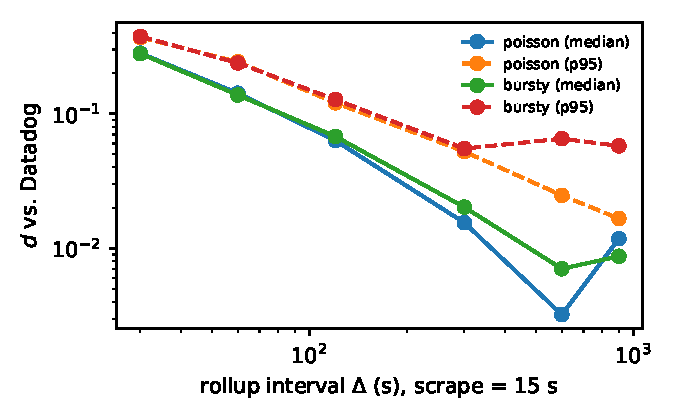
\includegraphics[width=0.6\linewidth]{figures/rate_error_vs_window}
\caption{Error of \texttt{rate()} against Datadog as the rollup interval grows, at a
$15$\,s scrape interval. \texttt{rate} is the only candidate whose error depends on the
data.}
\label{fig:rate-error}
\end{figure}

\subsubsection{The dual-write replay}
\label{sec:replay}

Everything to this point compares a PromQL candidate against our reading of Datadog's
rollup. That is a model, and a model is what \S\ref{sec:not-measured} warns the reader
about. This subsection closes the gap for the counter rules by running the dual-write
construction of this section literally: one stream of observations, written to both
systems, read back from both.

The stream is real. Counting the requests in a web-server access log into a scrape grid
gives a counter with the shape that \S\ref{sec:threats} says the synthetic workloads only
imitate: in the half hour used here the per-minute rate swings seventeenfold without
being asked to. We take the busiest half hour of the Kennedy Space Center HTTP logs of
July~1995~\citep{nasahttp}, count requests at a $15$\,s scrape interval into one counter
per HTTP status class, and write the cumulative series to Prometheus and its image under
$\phi_{\mathsf{zero}}$ --- the per-interval deltas --- to Datadog, at the same timestamps
(\texttt{scripts\slash replay\_dualwrite.py}).
The trace's publishers ask that it not be analysed beyond general traffic patterns, and
the parser enforces that rather than promising it: it keeps a timestamp and a status
class and discards the host and the request line, so what is replayed is a count of
requests per interval and nothing else. Timestamps are shifted to the present, because
Datadog's intake refuses points much older than an hour; the shape is real and the
absolute times are not.

\begin{table}[htbp]\centering\footnotesize
\begin{tabular}{@{}llrrr@{}}
\toprule
Scrape grid & PromQL candidate & Evaluated inside & On the edge & Max $d$ \\
\midrule
unaligned & \texttt{x - x offset $\Delta$} & 100.0\% & 100.0\% & 0 \\
 & \texttt{increase(x[$\Delta$] anchored)} & 100.0\% & 100.0\% & 0 \\
 & \texttt{rate(x[$\Delta$])} $\times\,\Delta$ & 20.2\% & 20.2\% & 1 \\
\addlinespace
aligned & \texttt{x - x offset $\Delta$} & 100.0\% & 27.4\% & 0 \\
 & \texttt{increase(x[$\Delta$] anchored)} & 100.0\% & 27.4\% & 0 \\
 & \texttt{rate(x[$\Delta$])} $\times\,\Delta$ & 20.2\% & 16.7\% & 1 \\
\addlinespace
\bottomrule
\end{tabular}

\caption{The dual-write replay: each candidate against \emph{Datadog}, bucket by bucket,
on a real request trace. ``Inside'' and ``on the edge'' are the two evaluation instants
of Remark~\ref{rem:closure}. $84$ comparisons per row.}
\label{tab:replay}
\end{table}

Table~\ref{tab:replay} is the result, and two things in it are worth separating.

The first is that both exact forms are exact --- against Datadog, not against a model of
it, on traffic nobody generated for the purpose. \texttt{rate} is not, at $20.2\%$ of
buckets on both grids, which is what \S\ref{sec:ingestion} has said throughout and what
the steady synthetic workload conceals by being steady. That figure used to read
$19$--$20\%$, a spread between the two grids that was not a property of either: the
replay script scored this one table by bit-identity where every other exactness column in
this paper uses a $10^{-12}$ relative bound, and one aligned bucket reading $236.0$
against $235.999\ldots$ counted as a disagreement.

The second is about the convention of Remark~\ref{rem:closure}, and it explains how that
convention came to be assumed wrongly for so long. On the unaligned grid --- a scrape
whose samples do not fall on rollup boundaries, which is what a jittered scrape produces
and therefore the ordinary case --- evaluating on the bucket's edge agrees with
evaluating inside it, on every bucket. Off a boundary the two half-open intervals contain
the same samples, so the closure is simply not observable. Snap the scrape grid onto the
rollup grid and the same comparison falls from $100\%$ to $27.4\%$. The error was
invisible in exactly the configuration real deployments have, and decisive in the one the
synthetic workloads of Table~\ref{tab:rollup-live} happen to use.

What this does not do is also worth stating. A request counter does not reset in half an
hour, so \texttt{COUNTER\_RESET} is not exercised here; the restart rows of
Table~\ref{tab:rollup-live} and the scripted reset of E1 (Remark~\ref{rem:rho}) are the
evidence for that case. It is one window of one
trace at one rollup interval. And it tests the counter rules, not translation coverage:
$\kappa$ is what it was.

\paragraph{What was assumed, and what is left.}
This section began with two facts about Datadog that its documentation does not settle,
and carried a third about its backend. None is still an assumption, and the two it began
with did not turn out the way they were guessed.

The reset policy $\rho$ is no longer among them either, and it is the one that was
settled twice: read from the agent's source and then put to a running agent, which
agreed with the reading (Remark~\ref{rem:rho}). It too went against the guess --- the
prediction recorded in advance was discarding the interval, which turns out not to be a
reset policy at all.

Bucket closure is no longer among them. Remark~\ref{rem:closure} settles it by
measurement: buckets are left-closed and named by their start, which is the opposite of
what an earlier draft of this section assumed and the opposite of PromQL's own
convention. Epoch alignment \emph{is} documented~\citep{ddrollup}, so the remaining
content of \texttt{ROLLUP\_ALIGNMENT} is sharper than ``align the grids'': a PromQL
window follows the evaluation step, and the step that reads a Datadog bucket is one
\emph{inside} its right edge rather than on it. Evaluating on the boundary --- the
obvious choice once the closure is known --- disagrees on every bucket where a scrape
lands on the boundary too, which is the ordinary case. The translator records
\texttt{ROLLUP\_ALIGNMENT} on every rollup it emits for that reason.

Nothing is left. The last of the three --- whether Datadog's backend stores what its
agent sends --- stood until a counter was made to reset on purpose, which is what the
replay above cannot do and what E1 does (Remark~\ref{rem:rho}). Both systems scrape one
endpoint across the reset; Datadog stores $103$ over the bucket holding it, and
\texttt{increase($x$[$60$s] anchored)} over Prometheus returns $103$ for the same bucket,
as it does on every complete bucket of all three counters. So the restart rows of
Table~\ref{tab:rollup-live} no longer stand alone: the anchored form tracks
$\phi_{\mathsf{zero}}$, and Datadog agrees with it where a counter actually restarts.
